\chapter{Feasibility of Learning}
\lecture{4}{23 Sep.}{}

\begin{prev}
    \autoref{sec:pla} produced a working learning model, and \autoref{sec:outspace}
    onwards mapped the settings around it. Every guarantee obtained so far ---
    PLA halts, PLA makes no mistake on \(\mathcal{D}\) --- is a statement about
    the examples we were handed.
\end{prev}

\(\mathcal{D}\) is not what we are paid for. The bank wants the next applicant
classified, not the ones already in its files, and nothing in the previous three
chapters connects the two. This chapter takes that gap seriously enough to argue
first that it cannot be bridged at all, and then that it can --- once we agree to
settle for a guarantee of a weaker kind. Four steps: a proof that learning is
impossible, a probabilistic escape, the escape applied to one hypothesis, and
finally to a whole hypothesis set.

\section{Learning is Impossible?}\label{sec:nfl}

\source{slides p.2--6}

\subsection{A Learning Puzzle}

Before any mathematics, a test of your own human learning, with six examples.

\begin{center}
    \begin{tikzpicture}[scale=0.36]
        \puzzleat{0}{4.4}{100101010}
        \puzzleat{4.4}{4.4}{100001101}
        \puzzleat{8.8}{4.4}{100001000}
        \node[right] at (12.6,5.9) {\(y_n = -1\)};
        \puzzleat{0}{0}{001010100}
        \puzzleat{4.4}{0}{010101010}
        \puzzleat{8.8}{0}{011110011}
        \node[right] at (12.6,1.5) {\(y_n = +1\)};
        \draw[black!75] (0,-1.5) -- (17.0,-1.5);
        \puzzleat{4.4}{-6.0}{100010001}
        \node[right] at (8.8,-4.5) {\(g(\bm{x}) = \,?\)};
    \end{tikzpicture}
\end{center}

Each \(\bm{x}_n\) is a \(3 \times 3\) picture of black and white cells; three of
them are labelled \(-1\) and three \(+1\). What does your \(g\) say about the
seventh?

\subsection{Two Controversial Answers}

Whatever you say about \(g(\bm{x})\), an answer with reasons behind it is
available for the other side as well.

\begin{center}
    \begin{tabular}{@{}p{0.46\linewidth}p{0.46\linewidth}@{}}
        \toprule
        \textbf{truth \(f(\bm{x}) = +1\) because \ldots} &
        \textbf{truth \(f(\bm{x}) = -1\) because \ldots}\\
        \midrule
        \begin{itemize}[leftmargin=*, nosep]
            \item symmetry \(\iff +1\);
            \item (black or white count \(= 3\)) or (black count \(= 4\) and
                middle-top black) \(\iff +1\).
        \end{itemize}
        &
        \begin{itemize}[leftmargin=*, nosep]
            \item left-top black \(\iff -1\);
            \item middle column contains at most \(1\) black and right-top white
                \(\iff -1\).
        \end{itemize}\\
        \addlinespace[4pt]
        \bottomrule
    \end{tabular}
\end{center}

\begin{observation}
    All four rules are correct on all six examples, and all four fire on the
    test picture. The last one is worth checking by hand: its main diagonal is
    black, so it is symmetric and its black count is \(3\), which the left-hand
    rules read as \(+1\); its left-top cell is black and its middle column holds
    one black with a white right-top cell, which the right-hand rules read as
    \(-1\).
\end{observation}

So the data does not decide. Any answer you give can be called wrong by a
teacher who had one of the other rules in mind all along, and that teacher never
has to admit to cheating --- the rule was consistent with everything you were
shown.

\begin{moral}
    All valid reasons: your adversarial teacher can always call you `didn't
    learn'. :-(
\end{moral}

\subsection{A `Simple' Binary Classification Problem}

The puzzle is easier to argue about once it is small enough to write out
completely. Take
\[
    \mathcal{X} = \left\{ 0, 1 \right\}^3 , \qquad
    \mathcal{Y} = \left\{ \circ, \times \right\} ,
\]
so that \(\mathcal{X}\) has eight points and there are only \(2^8 = 256\)
candidate targets \(f\) --- few enough that \(\mathcal{H}\) can be taken to be
\emph{all} of them. Suppose five of the eight points come to us labelled:

\begin{center}
    \begin{tabular}{@{}c|c@{}}
        \toprule
        \(\bm{x}_n\) & \(y_n = f(\bm{x}_n)\)\\
        \midrule
        \(0\,0\,0\) & \(\circ\)\\
        \(0\,0\,1\) & \(\times\)\\
        \(0\,1\,0\) & \(\times\)\\
        \(0\,1\,1\) & \(\circ\)\\
        \(1\,0\,0\) & \(\times\)\\
        \bottomrule
    \end{tabular}
\end{center}

\begin{question}
    Pick \(g \in \mathcal{H}\) with \(g(\bm{x}_n) = y_n\) for every \(n\), the
    way PLA does. Does \(g \approx f\)?
\end{question}

\subsection{No Free Lunch}

Fixing the five labels kills \(2^5\) of the \(256\) degrees of freedom and
leaves \(2^3 = 8\) targets standing. Here they are, next to any \(g\) we might
have picked.

\begin{center}
    \begin{adjustbox}{max width=\textwidth}
        \begin{tabular}{@{}c@{\ \ \ }c|c|c|cccccccc@{}}
            \toprule
            & \(\bm{x}\) & \(y\) & \(g\) & \(f_1\) & \(f_2\) & \(f_3\) & \(f_4\)
            & \(f_5\) & \(f_6\) & \(f_7\) & \(f_8\)\\
            \midrule
            \ldelim\{{5}{8mm}[\(\mathcal{D}\)\,]
            & \(000\) & \(\circ\) & \(\circ\) & \(\circ\) & \(\circ\) & \(\circ\) & \(\circ\) & \(\circ\) & \(\circ\) & \(\circ\) & \(\circ\)\\
            & \(001\) & \(\times\) & \(\times\) & \(\times\) & \(\times\) & \(\times\) & \(\times\) & \(\times\) & \(\times\) & \(\times\) & \(\times\)\\
            & \(010\) & \(\times\) & \(\times\) & \(\times\) & \(\times\) & \(\times\) & \(\times\) & \(\times\) & \(\times\) & \(\times\) & \(\times\)\\
            & \(011\) & \(\circ\) & \(\circ\) & \(\circ\) & \(\circ\) & \(\circ\) & \(\circ\) & \(\circ\) & \(\circ\) & \(\circ\) & \(\circ\)\\
            & \(100\) & \(\times\) & \(\times\) & \(\times\) & \(\times\) & \(\times\) & \(\times\) & \(\times\) & \(\times\) & \(\times\) & \(\times\)\\
            \midrule
            & \(101\) & & \(?\) & \(\circ\) & \(\circ\) & \(\circ\) & \(\circ\) & \(\times\) & \(\times\) & \(\times\) & \(\times\)\\
            & \(110\) & & \(?\) & \(\circ\) & \(\circ\) & \(\times\) & \(\times\) & \(\circ\) & \(\circ\) & \(\times\) & \(\times\)\\
            & \(111\) & & \(?\) & \(\circ\) & \(\times\) & \(\circ\) & \(\times\) & \(\circ\) & \(\times\) & \(\circ\) & \(\times\)\\
            \bottomrule
        \end{tabular}
    \end{adjustbox}
\end{center}

The top block is the same in every column, which is the good news:

\begin{itemize}
    \item \(g \approx f\) inside \(\mathcal{D}\): sure!
    \item \(g \approx f\) outside \(\mathcal{D}\): \textbf{No!} --- but that is
        really what we want.
\end{itemize}

The bottom block is the bad news, and it is as bad as it can be: for each of the
three unseen inputs, four of the surviving targets say \(\circ\) and four say
\(\times\). Whatever \(g\) fills into a `?', half of the candidates disagree
with it. This is worth saying once in general.

\begin{proposition}[No free lunch]\label{prop:nfl}
    Let \(\mathcal{H}\) contain every \(f\colon \mathcal{X} \to
    \left\{ -1, +1 \right\}\), let \(\mathcal{D}\) be any set of labelled
    examples, and let \(\bm{x} \notin \mathcal{D}\). Among the targets that
    agree with \(\mathcal{D}\), exactly half satisfy \(f(\bm{x}) = +1\) and half
    satisfy \(f(\bm{x}) = -1\). Consequently every algorithm, no matter how it
    computes \(g\), is wrong at \(\bm{x}\) for exactly half of them.
\end{proposition}

\begin{proof}
    Write \(S\) for the set of targets that agree with \(\mathcal{D}\) --- the
    eight columns of the table above, in the example. Given \(f \in S\), let
    \(f'\) be the target that copies \(f\) at every input except \(\bm{x}\),
    where it answers the other way: \(f'(\bm{x}) = -f(\bm{x})\).

    That \(f'\) is again in \(S\) is the one place the hypothesis
    \(\bm{x} \notin \mathcal{D}\) is used: the single value that was changed
    sits at \(\bm{x}\), which is not one of the examples, so \(f'\) still
    reproduces every label of \(\mathcal{D}\). Flipping twice returns the
    original, \((f')' = f\), and \(f'\) is never \(f\) itself, since the two
    differ at \(\bm{x}\) by construction. A rule that pairs each element with
    another one and is undone by applying it again leaves nobody over, so
    \(f \mapsto f'\) cuts \(S\) into pairs, and the two members of a pair give
    opposite answers at \(\bm{x}\).

    Half of \(S\) therefore answers \(+1\) at \(\bm{x}\) and half answers
    \(-1\). Now \(g(\bm{x})\) is a single fixed value, whatever \(\mathcal{A}\)
    did to arrive at it, so within each pair it agrees with one member and
    disagrees with the other.
\end{proof}

In the table, with \(\bm{x} = 101\), that pairing is
\(f_1 \leftrightarrow f_5\), \(f_2 \leftrightarrow f_6\),
\(f_3 \leftrightarrow f_7\), \(f_4 \leftrightarrow f_8\): the members of a pair
agree on every other row and differ only in that one.

The proof uses nothing about the algorithm --- it never appears --- which is
exactly why no cleverer \(\mathcal{A}\) can escape. The trouble is the
assumption that \(f\) is completely unrestricted.

\begin{moral}
    Learning from \(\mathcal{D}\) (to infer something outside \(\mathcal{D}\))
    is doomed if any `unknown' \(f\) can happen. :-(
\end{moral}

\begin{exercise}[Fun Time]
    This is a popular `brain-storming' problem, with a claim that \(2\%\) of the
    world's cleverest population can crack its `hidden pattern':
    \[
        (5, 3, 2) \to 151022, \qquad (7, 2, 5) \to \,?
    \]
    It is a learning problem with \(N = 1\), \(\bm{x}_1 = (5,3,2)\), \(y_1 =
    151022\). Learn a hypothesis from the one example to predict on
    \(\bm{x} = (7,2,5)\). What is your answer?
    \begin{enumerate}[(1)]
        \item \(151026\);
        \item \(143547\);
        \item I need more examples to get the correct answer;
        \item there is no `correct' answer.
    \end{enumerate}
\end{exercise}

\begin{proof}[Reference Answer]
    (4). Following the same nature of the no-free-lunch problems discussed, we
    cannot hope to be correct under this `adversarial' setting. The designer's
    answer is (2): the first two digits are \(x_1 \cdot x_2\), the next two
    \(x_1 \cdot x_3\), and the last two \(x_1 \cdot x_2 + x_1 \cdot x_3 - x_2\).
    Knowing that does not make (2) any more correct than (1) --- it only tells
    you which \(f\) this particular teacher had in mind.
\end{proof}

\section{Probability to the Rescue}\label{sec:hoeffding}

\source{slides p.7--12}

\subsection{Inferring Something Unknown}

\autoref{prop:nfl} closes one door: the unknown target \(f\) outside
\(\mathcal{D}\) cannot be inferred. Before giving up, it is worth asking whether
\emph{any} unknown quantity is ever inferred from a sample, in any other corner
of mathematics --- and one is, routinely.

Consider a bin holding very many marbles, each orange or green.

\begin{center}
    \begin{tikzpicture}
        \begin{scope}[scale=2.4]
            \node[mgreen=6.3pt] at (-0.276,0.048) {};
            \node[mgreen=6.3pt] at (-0.184,0.048) {};
            \node[morange=6.3pt] at (-0.092,0.048) {};
            \node[morange=6.3pt] at (0.000,0.048) {};
            \node[morange=6.3pt] at (0.092,0.048) {};
            \node[mgreen=6.3pt] at (0.184,0.048) {};
            \node[mgreen=6.3pt] at (0.276,0.048) {};
            \node[mgreen=6.3pt] at (-0.230,0.128) {};
            \node[morange=6.3pt] at (-0.138,0.128) {};
            \node[mgreen=6.3pt] at (-0.046,0.128) {};
            \node[mgreen=6.3pt] at (0.046,0.128) {};
            \node[mgreen=6.3pt] at (0.138,0.128) {};
            \node[mgreen=6.3pt] at (0.230,0.128) {};
            \node[mgreen=6.3pt] at (0.322,0.128) {};
            \node[mgreen=6.3pt] at (-0.368,0.208) {};
            \node[mgreen=6.3pt] at (-0.276,0.208) {};
            \node[mgreen=6.3pt] at (-0.184,0.208) {};
            \node[mgreen=6.3pt] at (-0.092,0.208) {};
            \node[mgreen=6.3pt] at (0.000,0.208) {};
            \node[mgreen=6.3pt] at (0.092,0.208) {};
            \node[morange=6.3pt] at (0.184,0.208) {};
            \node[morange=6.3pt] at (0.276,0.208) {};
            \node[mgreen=6.3pt] at (0.368,0.208) {};
            \node[mgreen=6.3pt] at (-0.230,0.287) {};
            \node[mgreen=6.3pt] at (-0.138,0.287) {};
            \node[mgreen=6.3pt] at (-0.046,0.287) {};
            \node[mgreen=6.3pt] at (0.046,0.287) {};
            \node[mgreen=6.3pt] at (0.138,0.287) {};
            \node[mgreen=6.3pt] at (0.230,0.287) {};
            \node[mgreen=6.3pt] at (0.322,0.287) {};
            \node[mgreen=6.3pt] at (-0.368,0.367) {};
            \node[morange=6.3pt] at (-0.276,0.367) {};
            \node[morange=6.3pt] at (-0.184,0.367) {};
            \node[mgreen=6.3pt] at (-0.092,0.367) {};
            \node[mgreen=6.3pt] at (0.000,0.367) {};
            \node[mgreen=6.3pt] at (0.092,0.367) {};
            \node[mgreen=6.3pt] at (0.184,0.367) {};
            \node[mgreen=6.3pt] at (0.276,0.367) {};
            \node[mgreen=6.3pt] at (0.368,0.367) {};
            \node[mgreen=6.3pt] at (-0.230,0.447) {};
            \node[morange=6.3pt] at (-0.138,0.447) {};
            \node[mgreen=6.3pt] at (-0.046,0.447) {};
            \node[mgreen=6.3pt] at (0.046,0.447) {};
            \node[mgreen=6.3pt] at (0.138,0.447) {};
            \node[mgreen=6.3pt] at (0.230,0.447) {};
            \node[morange=6.3pt] at (0.322,0.447) {};
            \node[mgreen=6.3pt] at (-0.276,0.526) {};
            \node[morange=6.3pt] at (-0.184,0.526) {};
            \node[morange=6.3pt] at (-0.092,0.526) {};
            \node[mgreen=6.3pt] at (0.000,0.526) {};
            \node[morange=6.3pt] at (0.092,0.526) {};
            \node[mgreen=6.3pt] at (0.184,0.526) {};
            \node[mgreen=6.3pt] at (0.276,0.526) {};
            \node[mgreen=6.3pt] at (-0.138,0.606) {};
            \node[mgreen=6.3pt] at (-0.046,0.606) {};
            \node[morange=6.3pt] at (0.046,0.606) {};
            \node[morange=6.3pt] at (0.138,0.606) {};
            \node[mgreen=6.3pt] at (0.230,0.606) {};
            \node[morange=6.3pt] at (-0.184,0.686) {};
            \node[morange=6.3pt] at (-0.092,0.686) {};
            \node[morange=6.3pt] at (0.000,0.686) {};
            \node[mgreen=6.3pt] at (0.092,0.686) {};
            \node[mgreen=6.3pt] at (0.184,0.686) {};
            \node[mgreen=6.3pt] at (-0.138,0.765) {};
            \node[morange=6.3pt] at (-0.046,0.765) {};
            \node[mgreen=6.3pt] at (0.046,0.765) {};
            \node[mgreen=6.3pt] at (0.138,0.765) {};
            \node[mgreen=6.3pt] at (0.230,0.765) {};
            \node[morange=6.3pt] at (-0.184,0.845) {};
            \node[mgreen=6.3pt] at (-0.092,0.845) {};
            \node[mgreen=6.3pt] at (0.000,0.845) {};
            \node[morange=6.3pt] at (0.092,0.845) {};
            \node[mgreen=6.3pt] at (0.184,0.845) {};
            \node[mgreen=6.3pt] at (-0.138,0.925) {};
            \node[mgreen=6.3pt] at (-0.046,0.925) {};
            \node[morange=6.3pt] at (0.046,0.925) {};
            \node[mgreen=6.3pt] at (0.138,0.925) {};
            \node[mgreen=6.3pt] at (0.230,0.925) {};
        \end{scope}
        \draw[binwall, scale=2.4] \binpath;
        \node[font=\small\bfseries, below] at (0,-0.12) {bin};
    \end{tikzpicture}
\end{center}

Do we \emph{know} what fraction of them is orange? No: nobody counted, and the
bin may hold more marbles than we could ever count.

\begin{question}
    Can you \emph{infer} the orange probability?
\end{question}

\subsection{Statistics 101: Inferring Orange Probability}

The statistician's move is to grab a handful without looking.

\begin{center}
    \begin{adjustbox}{max width=\textwidth}
        \begin{tikzpicture}
            \begin{scope}[scale=2.6]
            \node[mgreen=5.9pt] at (-0.320,0.042) {};
            \node[mgreen=5.9pt] at (-0.240,0.042) {};
            \node[mgreen=5.9pt] at (-0.160,0.042) {};
            \node[morange=5.9pt] at (-0.080,0.042) {};
            \node[morange=5.9pt] at (0.000,0.042) {};
            \node[mgreen=5.9pt] at (0.080,0.042) {};
            \node[morange=5.9pt] at (0.160,0.042) {};
            \node[mgreen=5.9pt] at (0.240,0.042) {};
            \node[mgreen=5.9pt] at (0.320,0.042) {};
            \node[mgreen=5.9pt] at (-0.280,0.111) {};
            \node[morange=5.9pt] at (-0.200,0.111) {};
            \node[morange=5.9pt] at (-0.120,0.111) {};
            \node[morange=5.9pt] at (-0.040,0.111) {};
            \node[mgreen=5.9pt] at (0.040,0.111) {};
            \node[mgreen=5.9pt] at (0.120,0.111) {};
            \node[mgreen=5.9pt] at (0.200,0.111) {};
            \node[mgreen=5.9pt] at (0.280,0.111) {};
            \node[mgreen=5.9pt] at (0.360,0.111) {};
            \node[mgreen=5.9pt] at (-0.320,0.181) {};
            \node[mgreen=5.9pt] at (-0.240,0.181) {};
            \node[morange=5.9pt] at (-0.160,0.181) {};
            \node[morange=5.9pt] at (-0.080,0.181) {};
            \node[mgreen=5.9pt] at (0.000,0.181) {};
            \node[morange=5.9pt] at (0.080,0.181) {};
            \node[morange=5.9pt] at (0.160,0.181) {};
            \node[mgreen=5.9pt] at (0.240,0.181) {};
            \node[mgreen=5.9pt] at (0.320,0.181) {};
            \node[mgreen=5.9pt] at (-0.280,0.250) {};
            \node[mgreen=5.9pt] at (-0.200,0.250) {};
            \node[mgreen=5.9pt] at (-0.120,0.250) {};
            \node[mgreen=5.9pt] at (-0.040,0.250) {};
            \node[morange=5.9pt] at (0.040,0.250) {};
            \node[morange=5.9pt] at (0.120,0.250) {};
            \node[morange=5.9pt] at (0.200,0.250) {};
            \node[mgreen=5.9pt] at (0.280,0.250) {};
            \node[morange=5.9pt] at (0.360,0.250) {};
            \node[mgreen=5.9pt] at (-0.320,0.319) {};
            \node[morange=5.9pt] at (-0.240,0.319) {};
            \node[mgreen=5.9pt] at (-0.160,0.319) {};
            \node[morange=5.9pt] at (-0.080,0.319) {};
            \node[morange=5.9pt] at (0.000,0.319) {};
            \node[mgreen=5.9pt] at (0.080,0.319) {};
            \node[mgreen=5.9pt] at (0.160,0.319) {};
            \node[mgreen=5.9pt] at (0.240,0.319) {};
            \node[mgreen=5.9pt] at (0.320,0.319) {};
            \node[mgreen=5.9pt] at (-0.280,0.388) {};
            \node[morange=5.9pt] at (-0.200,0.388) {};
            \node[mgreen=5.9pt] at (-0.120,0.388) {};
            \node[mgreen=5.9pt] at (-0.040,0.388) {};
            \node[mgreen=5.9pt] at (0.040,0.388) {};
            \node[mgreen=5.9pt] at (0.120,0.388) {};
            \node[mgreen=5.9pt] at (0.200,0.388) {};
            \node[morange=5.9pt] at (0.280,0.388) {};
            \node[mgreen=5.9pt] at (0.360,0.388) {};
            \node[morange=5.9pt] at (-0.320,0.458) {};
            \node[morange=5.9pt] at (-0.240,0.458) {};
            \node[mgreen=5.9pt] at (-0.160,0.458) {};
            \node[mgreen=5.9pt] at (-0.080,0.458) {};
            \node[mgreen=5.9pt] at (0.000,0.458) {};
            \node[mgreen=5.9pt] at (0.080,0.458) {};
            \node[mgreen=5.9pt] at (0.160,0.458) {};
            \node[mgreen=5.9pt] at (0.240,0.458) {};
            \node[mgreen=5.9pt] at (0.320,0.458) {};
            \node[morange=5.9pt] at (-0.200,0.527) {};
            \node[mgreen=5.9pt] at (-0.120,0.527) {};
            \node[morange=5.9pt] at (-0.040,0.527) {};
            \node[mgreen=5.9pt] at (0.040,0.527) {};
            \node[morange=5.9pt] at (0.120,0.527) {};
            \node[mgreen=5.9pt] at (0.200,0.527) {};
            \node[morange=5.9pt] at (0.280,0.527) {};
            \node[mgreen=5.9pt] at (-0.240,0.596) {};
            \node[morange=5.9pt] at (-0.160,0.596) {};
            \node[mgreen=5.9pt] at (-0.080,0.596) {};
            \node[mgreen=5.9pt] at (0.000,0.596) {};
            \node[morange=5.9pt] at (0.080,0.596) {};
            \node[mgreen=5.9pt] at (0.160,0.596) {};
            \node[mgreen=5.9pt] at (0.240,0.596) {};
            \node[mgreen=5.9pt] at (-0.200,0.666) {};
            \node[mgreen=5.9pt] at (-0.120,0.666) {};
            \node[morange=5.9pt] at (-0.040,0.666) {};
            \node[morange=5.9pt] at (0.040,0.666) {};
            \node[mgreen=5.9pt] at (0.120,0.666) {};
            \node[mgreen=5.9pt] at (0.200,0.666) {};
            \node[morange=5.9pt] at (0.280,0.666) {};
            \node[mgreen=5.9pt] at (-0.240,0.735) {};
            \node[mgreen=5.9pt] at (-0.160,0.735) {};
            \node[mgreen=5.9pt] at (-0.080,0.735) {};
            \node[mgreen=5.9pt] at (0.000,0.735) {};
            \node[mgreen=5.9pt] at (0.080,0.735) {};
            \node[morange=5.9pt] at (0.160,0.735) {};
            \node[morange=5.9pt] at (0.240,0.735) {};
            \node[mgreen=5.9pt] at (-0.120,0.804) {};
            \node[mgreen=5.9pt] at (-0.040,0.804) {};
            \node[mgreen=5.9pt] at (0.040,0.804) {};
            \node[morange=5.9pt] at (0.120,0.804) {};
            \node[mgreen=5.9pt] at (0.200,0.804) {};
            \node[morange=5.9pt] at (-0.240,0.873) {};
            \node[mgreen=5.9pt] at (-0.160,0.873) {};
            \node[morange=5.9pt] at (-0.080,0.873) {};
            \node[morange=5.9pt] at (0.000,0.873) {};
            \node[mgreen=5.9pt] at (0.080,0.873) {};
            \node[mgreen=5.9pt] at (0.160,0.873) {};
            \node[mgreen=5.9pt] at (0.240,0.873) {};
            \node[mgreen=5.9pt] at (-0.200,0.943) {};
            \node[mgreen=5.9pt] at (-0.120,0.943) {};
            \node[morange=5.9pt] at (-0.040,0.943) {};
            \node[mgreen=5.9pt] at (0.040,0.943) {};
            \node[mgreen=5.9pt] at (0.120,0.943) {};
            \node[mgreen=5.9pt] at (0.200,0.943) {};
            \node[mgreen=5.9pt] at (0.280,0.943) {};
            \end{scope}
            \draw[binwall, scale=2.6] \binpath;
            \node[font=\small\bfseries, below] at (0,-0.12) {bin};
            \draw[scoop] (0.15,2.70) .. controls (1.15,3.55) and (2.55,3.15) ..
                (3.15,1.80);
            \node[font=\small\bfseries] at (1.75,3.55) {sample of size \(N\)};
            \node[mgreen=5.9pt] at (3.35,1.55) {};
            \node[morange=5.9pt] at (3.56,1.55) {};
            \node[mgreen=5.9pt] at (3.77,1.55) {};
            \node[mgreen=5.9pt] at (3.98,1.55) {};
            \node[morange=5.9pt] at (4.19,1.55) {};
            \node[mgreen=5.9pt] at (4.40,1.55) {};
            \node[mgreen=5.9pt] at (4.61,1.55) {};
            \node[morange=5.9pt] at (4.82,1.55) {};
            \node[mgreen=5.9pt] at (5.03,1.55) {};
            \node[mgreen=5.9pt] at (5.24,1.55) {};
            \node[left, font=\small, align=right] at (-1.30,1.50)
                {\(\mu =\) orange\\probability in bin};
            \node[right, font=\small, align=left] at (5.70,1.55)
                {\(\nu =\) orange\\fraction in sample};
        \end{tikzpicture}
    \end{adjustbox}
\end{center}

\begin{notation}\label{not:munu}
    \(\mu\) is the orange probability in the bin and \(1 - \mu\) the green one;
    \(\mu\) is \textbf{unknown}. Draw \(N\) marbles independently, each with
    replacement, and let \(\nu\) be the orange fraction in that sample, \(1 -
    \nu\) the green one; \(\nu\) is \textbf{known}, because it is sitting in
    front of us. `In-sample' always refers to \(\nu\), `out-of-sample' to
    \(\mu\).
\end{notation}

\begin{question}
    Does the in-sample \(\nu\) say anything about the out-of-sample \(\mu\)?
\end{question}

\subsection{Possible versus Probable}

The answer has to be given twice, because the two obvious readings of the
question have opposite answers.

\begin{center}
    \begin{tabular}{@{}p{0.46\linewidth}p{0.46\linewidth}@{}}
        \toprule
        \textbf{No!} & \textbf{Yes!}\\
        \midrule
        Possibly not: the sample can come out mostly green while the bin is
        mostly orange. &
        Probably yes: the in-sample \(\nu\) is likely to be close to the unknown
        \(\mu\).\\
        \addlinespace[3pt]
        \bottomrule
    \end{tabular}
\end{center}

Note how little the two claims have to do with each other. The left column is
about what a sample \emph{can} be, and a bin of a million marbles of which
\(999{,}999\) are orange can still deliver ten green ones. The right column is
about what a sample \emph{tends} to be, and puts a number on `tends'. Nothing is
being hidden: the bad sample really does exist, we are simply going to bound how
often it turns up.

\begin{question}
    Formally, what does \(\nu\) say about \(\mu\)?
\end{question}

\subsection{Hoeffding's Inequality}

\begin{theorem}[Hoeffding's inequality]\label{thm:hoeffding}
    Draw \(N\) marbles independently from a bin whose orange probability is
    \(\mu\), and let \(\nu\) be the orange fraction among them. For every
    \(\epsilon > 0\),
    \[
        \mathbb{P}\left[ \abs{\nu - \mu} > \epsilon \right]
        \le 2 \exp \left( -2 \epsilon^2 N \right) .
    \]
\end{theorem}

The statement is about marbles, coins, polling and anything else that can be
sampled, and the three properties that make it usable are worth separating out.

\begin{itemize}
    \item It is valid for all \(N\) and all \(\epsilon\) --- no `\(N\) large
        enough' clause, no asymptotics.
    \item It does not depend on \(\mu\). We never need to `know' \(\mu\), which
        is the whole point, since \(\mu\) is what we are trying to infer.
    \item A larger sample size \(N\), or a looser gap \(\epsilon\), gives a
        higher probability for `\(\nu \approx \mu\)'.
\end{itemize}

\begin{definition}[PAC]
    A statement is \vocab{probably approximately correct} (PAC) when it may be
    off by a little (\emph{approximately}, the \(\epsilon\)) and may fail
    outright now and then (\emph{probably}, the bound on the right). The
    statement `\(\nu = \mu\)' is PAC.
\end{definition}

\begin{remark}
    The factor \(2\) is a union bound over the two ways of being wrong. Hoeffding
    proves \(\mathbb{P}\left[ \nu - \mu > \epsilon \right] \le
    \exp(-2\epsilon^2 N)\) and, by the same argument applied to green,
    \(\mathbb{P}\left[ \mu - \nu > \epsilon \right] \le \exp(-2\epsilon^2 N)\);
    adding the two gives the two-sided form. The same cheap trick --- bound each
    bad event, then add --- reappears in \autoref{sec:real-learning}, where it
    is the only tool used.
\end{remark}

\begin{note}
    The exponent decays in \(N\), so the bound is far better than its shape
    suggests. At \(\epsilon = 0.1\) and \(N = 1{,}000\) it reads
    \(2\exp(-20) \approx 4 \times 10^{-9}\): a thousand marbles pin down the
    contents of an arbitrarily large bin to within ten percentage points, and
    the chance of being fooled is one in a quarter of a billion.
\end{note}

\begin{moral}
    If \(N\) is large, we can probably infer the unknown \(\mu\) from the known
    \(\nu\).
\end{moral}

\begin{exercise}[Fun Time]
    Let \(\mu = 0.4\). Use Hoeffding's inequality to bound the probability that
    a sample of \(10\) marbles will have \(\nu \le 0.1\). What bound do you get?
    \begin{enumerate}[(1)]
        \item \(0.67\);
        \item \(0.40\);
        \item \(0.33\);
        \item \(0.05\).
    \end{enumerate}
\end{exercise}

\begin{proof}[Reference Answer]
    (3). The event \(\nu \le 0.1\) is contained in \(\abs{\nu - \mu} \ge 0.3\),
    so set \(N = 10\) and \(\epsilon = 0.3\):
    \[
        2 \exp \left( -2 (0.3)^2 (10) \right) = 2 e^{-1.8} \approx 0.33 .
    \]
    The actual probability is about \(0.05\), which is answer (4); Hoeffding
    gives only an upper bound, and at \(N = 10\) it is a loose one.
\end{proof}

\section{Connection to Learning}\label{sec:bin-learning}

\source{slides p.13--18}

\subsection{The Bin Analogy}

The bin is not an analogy chosen for decoration; every one of its pieces has a
counterpart in learning, and the translation is exact.

\begin{center}
    \begin{tabular}{@{}p{0.42\linewidth}p{0.52\linewidth}@{}}
        \toprule
        \textbf{bin} & \textbf{learning}\\
        \midrule
        unknown orange probability \(\mu\)
        & a \emph{fixed} hypothesis \(h(\bm{x})\), asked whether it equals the
        target \(f(\bm{x})\)\\[4pt]
        a marble \(\bullet\) in the bin & a point \(\bm{x} \in \mathcal{X}\)\\[4pt]
        \textcolor{marbleorange}{orange} marble
        & \(h\) is \textcolor{marbleorange}{wrong}: \(h(\bm{x}) \neq f(\bm{x})\)\\[4pt]
        \textcolor{marblegreen}{green} marble
        & \(h\) is \textcolor{marblegreen}{right}: \(h(\bm{x}) = f(\bm{x})\)\\[4pt]
        a size-\(N\) sample of i.i.d.\ marbles
        & checking \(h\) on \(\mathcal{D} = \left\{ (\bm{x}_n,
        \underbrace{y_n}_{f(\bm{x}_n)}) \right\}\) with i.i.d.\ \(\bm{x}_n\)\\
        \addlinespace[5pt]
        \bottomrule
    \end{tabular}
\end{center}

So the input space itself is the bin, and it is \(h\) that colours it: paint
\(\bm{x}\) orange where \(h\) disagrees with \(f\) and green where it agrees.

\begin{center}
    \begin{adjustbox}{max width=\textwidth}
        \begin{tikzpicture}
            \begin{scope}[scale=2.6]
            \node[mgreen=5.9pt] at (-0.320,0.042) {};
            \node[mgreen=5.9pt] at (-0.240,0.042) {};
            \node[morange=5.9pt] at (-0.160,0.042) {};
            \node[morange=5.9pt] at (-0.080,0.042) {};
            \node[mgreen=5.9pt] at (0.000,0.042) {};
            \node[mgreen=5.9pt] at (0.080,0.042) {};
            \node[morange=5.9pt] at (0.160,0.042) {};
            \node[morange=5.9pt] at (0.240,0.042) {};
            \node[mgreen=5.9pt] at (0.320,0.042) {};
            \node[mgreen=5.9pt] at (-0.280,0.111) {};
            \node[mgreen=5.9pt] at (-0.200,0.111) {};
            \node[mgreen=5.9pt] at (-0.120,0.111) {};
            \node[morange=5.9pt] at (-0.040,0.111) {};
            \node[mgreen=5.9pt] at (0.040,0.111) {};
            \node[mgreen=5.9pt] at (0.120,0.111) {};
            \node[mgreen=5.9pt] at (0.200,0.111) {};
            \node[mgreen=5.9pt] at (0.280,0.111) {};
            \node[mgreen=5.9pt] at (0.360,0.111) {};
            \node[mgreen=5.9pt] at (-0.320,0.181) {};
            \node[mgreen=5.9pt] at (-0.240,0.181) {};
            \node[morange=5.9pt] at (-0.160,0.181) {};
            \node[mgreen=5.9pt] at (-0.080,0.181) {};
            \node[mgreen=5.9pt] at (0.000,0.181) {};
            \node[mgreen=5.9pt] at (0.080,0.181) {};
            \node[mgreen=5.9pt] at (0.160,0.181) {};
            \node[morange=5.9pt] at (0.240,0.181) {};
            \node[mgreen=5.9pt] at (0.320,0.181) {};
            \node[morange=5.9pt] at (-0.280,0.250) {};
            \node[mgreen=5.9pt] at (-0.200,0.250) {};
            \node[mgreen=5.9pt] at (-0.120,0.250) {};
            \node[mgreen=5.9pt] at (-0.040,0.250) {};
            \node[mgreen=5.9pt] at (0.040,0.250) {};
            \node[mgreen=5.9pt] at (0.120,0.250) {};
            \node[mgreen=5.9pt] at (0.200,0.250) {};
            \node[mgreen=5.9pt] at (0.280,0.250) {};
            \node[morange=5.9pt] at (0.360,0.250) {};
            \node[morange=5.9pt] at (-0.320,0.319) {};
            \node[mgreen=5.9pt] at (-0.240,0.319) {};
            \node[mgreen=5.9pt] at (-0.160,0.319) {};
            \node[mgreen=5.9pt] at (-0.080,0.319) {};
            \node[mgreen=5.9pt] at (0.000,0.319) {};
            \node[morange=5.9pt] at (0.080,0.319) {};
            \node[mgreen=5.9pt] at (0.160,0.319) {};
            \node[mgreen=5.9pt] at (0.240,0.319) {};
            \node[mgreen=5.9pt] at (0.320,0.319) {};
            \node[mgreen=5.9pt] at (-0.280,0.388) {};
            \node[mgreen=5.9pt] at (-0.200,0.388) {};
            \node[mgreen=5.9pt] at (-0.120,0.388) {};
            \node[morange=5.9pt] at (-0.040,0.388) {};
            \node[mgreen=5.9pt] at (0.040,0.388) {};
            \node[mgreen=5.9pt] at (0.120,0.388) {};
            \node[mgreen=5.9pt] at (0.200,0.388) {};
            \node[mgreen=5.9pt] at (0.280,0.388) {};
            \node[mgreen=5.9pt] at (0.360,0.388) {};
            \node[mgreen=5.9pt] at (-0.320,0.458) {};
            \node[morange=5.9pt] at (-0.240,0.458) {};
            \node[mgreen=5.9pt] at (-0.160,0.458) {};
            \node[mgreen=5.9pt] at (-0.080,0.458) {};
            \node[morange=5.9pt] at (0.000,0.458) {};
            \node[mgreen=5.9pt] at (0.080,0.458) {};
            \node[mgreen=5.9pt] at (0.160,0.458) {};
            \node[mgreen=5.9pt] at (0.240,0.458) {};
            \node[mgreen=5.9pt] at (0.320,0.458) {};
            \node[mgreen=5.9pt] at (-0.200,0.527) {};
            \node[mgreen=5.9pt] at (-0.120,0.527) {};
            \node[morange=5.9pt] at (-0.040,0.527) {};
            \node[morange=5.9pt] at (0.040,0.527) {};
            \node[mgreen=5.9pt] at (0.120,0.527) {};
            \node[mgreen=5.9pt] at (0.200,0.527) {};
            \node[morange=5.9pt] at (0.280,0.527) {};
            \node[mgreen=5.9pt] at (-0.240,0.596) {};
            \node[morange=5.9pt] at (-0.160,0.596) {};
            \node[mgreen=5.9pt] at (-0.080,0.596) {};
            \node[mgreen=5.9pt] at (0.000,0.596) {};
            \node[mgreen=5.9pt] at (0.080,0.596) {};
            \node[mgreen=5.9pt] at (0.160,0.596) {};
            \node[morange=5.9pt] at (0.240,0.596) {};
            \node[mgreen=5.9pt] at (-0.200,0.666) {};
            \node[morange=5.9pt] at (-0.120,0.666) {};
            \node[mgreen=5.9pt] at (-0.040,0.666) {};
            \node[mgreen=5.9pt] at (0.040,0.666) {};
            \node[mgreen=5.9pt] at (0.120,0.666) {};
            \node[mgreen=5.9pt] at (0.200,0.666) {};
            \node[mgreen=5.9pt] at (0.280,0.666) {};
            \node[mgreen=5.9pt] at (-0.240,0.735) {};
            \node[mgreen=5.9pt] at (-0.160,0.735) {};
            \node[morange=5.9pt] at (-0.080,0.735) {};
            \node[mgreen=5.9pt] at (0.000,0.735) {};
            \node[morange=5.9pt] at (0.080,0.735) {};
            \node[mgreen=5.9pt] at (0.160,0.735) {};
            \node[morange=5.9pt] at (0.240,0.735) {};
            \node[morange=5.9pt] at (-0.120,0.804) {};
            \node[mgreen=5.9pt] at (-0.040,0.804) {};
            \node[mgreen=5.9pt] at (0.040,0.804) {};
            \node[morange=5.9pt] at (0.120,0.804) {};
            \node[morange=5.9pt] at (0.200,0.804) {};
            \node[morange=5.9pt] at (-0.240,0.873) {};
            \node[mgreen=5.9pt] at (-0.160,0.873) {};
            \node[mgreen=5.9pt] at (-0.080,0.873) {};
            \node[mgreen=5.9pt] at (0.000,0.873) {};
            \node[mgreen=5.9pt] at (0.080,0.873) {};
            \node[mgreen=5.9pt] at (0.160,0.873) {};
            \node[morange=5.9pt] at (0.240,0.873) {};
            \node[morange=5.9pt] at (-0.200,0.943) {};
            \node[mgreen=5.9pt] at (-0.120,0.943) {};
            \node[mgreen=5.9pt] at (-0.040,0.943) {};
            \node[mgreen=5.9pt] at (0.040,0.943) {};
            \node[mgreen=5.9pt] at (0.120,0.943) {};
            \node[morange=5.9pt] at (0.200,0.943) {};
            \node[mgreen=5.9pt] at (0.280,0.943) {};
            \end{scope}
            \draw[binwall, scale=2.6] \binpath;
            \node[font=\fontsize{46}{46}\selectfont] at (0,1.20) {\(\bm{\mathcal{X}}\)};
            \draw[scoop] (-0.18,2.42) .. controls (0.70,3.05) and (1.55,2.90) ..
                (2.30,2.66);
            \draw[scoop] (0.55,2.30) .. controls (1.20,2.45) and (1.70,2.25) ..
                (2.30,2.06);
            \node[morange=5.9pt] at (2.50,2.62) {};
            \node[right, font=\small] at (2.70,2.62)
                {\(h(\bm{x}) \neq f(\bm{x})\)};
            \node[mgreen=5.9pt] at (2.50,2.05) {};
            \node[right, font=\small] at (2.70,2.05)
                {\(h(\bm{x}) = f(\bm{x})\)};
        \end{tikzpicture}
    \end{adjustbox}
\end{center}

Two conditions make the translation legal, and they are exactly the two that
\autoref{thm:hoeffding} needs. The \(\bm{x}_n\) must be drawn independently, and
from the same distribution that will later produce the \(\bm{x}\) we are judged
on. Nothing is assumed about \emph{which} distribution that is.

\begin{moral}
    If \(N\) is large and the \(\bm{x}_n\) are i.i.d., we can probably infer the
    unknown \(\llbracket h(\bm{x}) \neq f(\bm{x}) \rrbracket\) probability from
    the known \(\llbracket h(\bm{x}_n) \neq y_n \rrbracket\) fraction.
\end{moral}

\subsection{Added Components}

The learning flow of \autoref{sec:components} therefore gains one box it did not
have: a probability distribution \(P\) on \(\mathcal{X}\), which generates both
the training inputs and the future ones.

\begin{center}
    \begin{adjustbox}{max width=\textwidth}
        \begin{tikzpicture}
            \node[mlbox, minimum width=4.4cm] (f) at (0,2.5)
                {unknown target function\\
                 \(f\colon \mathcal{X} \to \mathcal{Y}\)\\[2pt]
                 {\scriptsize (ideal credit approval formula)}};
            \node[mlbox, minimum width=2.6cm, draw=Dandelion!80!black,
                fill=Dandelion!12] (P) at (5.4,2.5)
                {unknown\\\(P\) on \(\mathcal{X}\)};
            \node[mlbox, minimum width=2.2cm, draw=Dandelion!80!black,
                fill=Dandelion!12] (test) at (10.2,2.5)
                {\(h \stackrel{?}{\approx} f\)};
            \node[mlbox, minimum width=5.2cm] (D) at (0,0)
                {training examples\\
                 \(\mathcal{D}\colon (\bm{x}_1, y_1), \dots , (\bm{x}_N, y_N)\)\\[2pt]
                 {\scriptsize (historical records in bank)}};
            \node[mlop, minimum width=2.4cm] (A) at (5.4,0)
                {learning\\algorithm\\\(\mathcal{A}\)};
            \node[mlbox, minimum width=4.4cm] (g) at (10.2,0)
                {final hypothesis\\\(g \approx f\)\\[2pt]
                 {\scriptsize (`learned' formula to be used)}};
            \node[mlbox, minimum width=3.4cm] (H) at (5.4,-2.4)
                {hypothesis set\\\(\mathcal{H}\)\\[2pt]
                 {\scriptsize (set of candidate formulas)}};
            \node[mlbox, minimum width=1.8cm, draw=Dandelion!80!black,
                fill=Dandelion!12] (fh) at (10.2,-2.4) {fixed \(h\)};
            \draw[mlarrow] (f) -- (D);
            \draw[mlarrow, draw=Dandelion!80!black, dashed] (P) -- (D)
                node[pos=0.58, font=\scriptsize, fill=white, inner sep=1.5pt]
                {\(\bm{x}_1, \bm{x}_2, \dots , \bm{x}_N\)};
            \draw[mlarrow, draw=Dandelion!80!black, dashed] (P) -- (test)
                node[midway, above, font=\scriptsize] {\(\bm{x}\)};
            \draw[mlarrow] (D) -- (A);
            \draw[mlarrow] (A) -- (g);
            \draw[mlarrow] (H) -- (A);
            \draw[mlarrow, draw=Dandelion!80!black] (H) -- (fh);
            \draw[mlarrow, draw=Dandelion!80!black] (fh.east)
                .. controls (13.8,-2.4) and (13.8,2.5) .. (test.east);
        \end{tikzpicture}
    \end{adjustbox}
\end{center}

The two quantities the bin analogy named now have proper symbols.

\begin{definition}[In-sample and out-of-sample error]\label{def:errors}
    For a hypothesis \(h\), the \vocab{out-of-sample error}
    \[
        \Eout(h) = \mathop{\mathcal{E}}_{\bm{x} \sim P}
        \llbracket h(\bm{x}) \neq f(\bm{x}) \rrbracket
    \]
    is the probability that \(h\) is wrong on a fresh input, and the
    \vocab{in-sample error}
    \[
        \Ein(h) = \frac{1}{N} \sum_{n=1}^{N}
        \llbracket h(\bm{x}_n) \neq y_n \rrbracket
    \]
    is the fraction of the examples it gets wrong. In the bin picture
    \(\Eout(h)\) is \(\mu\) and \(\Ein(h)\) is \(\nu\).
\end{definition}

\begin{moral}
    For any fixed \(h\), we can probably infer the unknown \(\Eout(h)\) from the
    known \(\Ein(h)\).
\end{moral}

\subsection{The Formal Guarantee}

Rewriting \autoref{thm:hoeffding} in this notation costs nothing and says
everything.

\begin{theorem}[Hoeffding for a fixed hypothesis]\label{thm:hoeffding-h}
    Fix \(h\) before seeing \(\mathcal{D}\), and let the \(\bm{x}_n\) be drawn
    i.i.d.\ from \(P\). Then for every \(\epsilon > 0\),
    \[
        \mathbb{P}\left[ \abs{\Ein(h) - \Eout(h)} > \epsilon \right]
        \le 2 \exp \left( -2 \epsilon^2 N \right) .
    \]
\end{theorem}

The same three remarks as before apply, and the third one has teeth here.

\begin{itemize}
    \item Valid for all \(N\) and \(\epsilon\).
    \item Does not depend on \(\Eout(h)\), so there is no need to `know'
        \(\Eout(h)\): both \(f\) and \(P\) may stay unknown.
    \item `\(\Ein(h) = \Eout(h)\)' is probably approximately correct.
\end{itemize}

\begin{moral}
    If `\(\Ein(h) \approx \Eout(h)\)' and `\(\Ein(h)\) small', then
    \(\Eout(h)\) is small, i.e.\ \(h \approx f\) with respect to \(P\).
\end{moral}

That last line deserves to be read slowly, because it says what \(g \approx f\)
has meant all along. It is not `\(g\) and \(f\) agree everywhere' --- no amount
of data can buy that, by \autoref{prop:nfl}. It is `\(g\) and \(f\) agree on
inputs that actually occur', weighted by how often they occur. Regions of
\(\mathcal{X}\) that \(P\) never visits are free to disagree, and we never find
out.

\subsection{Verification of One \texorpdfstring{\(h\)}{h}}

So for any fixed \(h\), when the data is large enough, \(\Ein(h) \approx
\Eout(h)\). Learning, however, never reports an \(h\) of our choosing: it
reports \(g = \mathcal{A}(\mathcal{D})\), the single hypothesis the algorithm
settles on out of \(\mathcal{H}\) after seeing \(\mathcal{D}\).

\begin{question}
    Can we then claim `good learning', that is, \(g \approx f\) for the
    \(g = \mathcal{A}(\mathcal{D})\) the algorithm actually returns?
\end{question}

\begin{center}
    \begin{tabular}{@{}p{0.46\linewidth}p{0.46\linewidth}@{}}
        \toprule
        \textbf{Yes!} & \textbf{No!}\\
        \midrule
        If \(\Ein(h)\) is small for the fixed \(h\), and \(\mathcal{A}\) picks
        that \(h\) as \(g\), then `\(g = f\)' is PAC. &
        If \(\mathcal{A}\) is \emph{forced} to pick THE \(h\) as \(g\), then
        \(\Ein(h)\) is almost always not small, and `\(g \neq f\)' is PAC!\\
        \addlinespace[3pt]
        \bottomrule
    \end{tabular}
\end{center}

Both columns describe the same arrangement --- one \(h\) nominated before the
data, returned as \(g\) --- and differ only in whether \(\Ein(h)\) turns out
small, which is not ours to arrange: an \(h\) written down before anyone looks
at \(\mathcal{D}\) has no reason to fit it. So \(\Ein(h)\) is almost always
large, \autoref{thm:hoeffding-h} carries \emph{that} over to \(\Eout(h)\) just
as faithfully, and what gets PAC-certified is `\(g \neq f\)'. The theorem does
not fail us; it works perfectly and reports that we are reliably wrong. The
obvious repair --- read \(\mathcal{D}\) first, then return whichever \(h\) fits
it --- is precisely what the premise `fix \(h\) before seeing \(\mathcal{D}\)'
rules out. Reading the data was never the problem, since \(\Ein(h)\) is computed
from it; the problem is that an \(h\) chosen that way is a function of
\(\mathcal{D}\), so it names no one bin whose \(\mu\) stood fixed while the
sample was drawn, and \autoref{thm:hoeffding-h} has nothing to say about it.

\begin{moral}
    Real learning: \(\mathcal{A}\) shall make choices \(\in \mathcal{H}\) (like
    PLA), rather than being forced to pick one \(h\). :-(
\end{moral}

\subsection{The `Verification' Flow}

What \autoref{thm:hoeffding-h} does buy is a complete and genuinely useful
procedure, one step short of learning. Somebody hands you a formula; you check
it against historical records; Hoeffding tells you how much the check is worth.

\begin{center}
    \begin{adjustbox}{max width=\textwidth}
        \begin{tikzpicture}
            \node[mlbox, minimum width=4.4cm] (f) at (0,2.5)
                {unknown target function\\
                 \(f\colon \mathcal{X} \to \mathcal{Y}\)\\[2pt]
                 {\scriptsize (ideal credit approval formula)}};
            \node[mlbox, minimum width=2.6cm, draw=Dandelion!80!black,
                fill=Dandelion!12] (P) at (5.0,2.5)
                {unknown\\\(P\) on \(\mathcal{X}\)};
            \node[mlbox, minimum width=5.2cm] (D) at (0,0)
                {verifying examples\\
                 \(\mathcal{D}\colon (\bm{x}_1, y_1), \dots , (\bm{x}_N, y_N)\)\\[2pt]
                 {\scriptsize (historical records in bank)}};
            \node[mlbox, minimum width=4.4cm] (g) at (9.2,0)
                {final hypothesis\\\(g \approx f\)\\[2pt]
                 {\scriptsize (given formula to be verified)}};
            \node[mlbox, minimum width=3.0cm] (h) at (4.4,-2.4)
                {one hypothesis\\\(h\)\\[2pt]
                 {\scriptsize (one candidate formula)}};
            \draw[mlarrow] (f) -- (D);
            \draw[mlarrow, draw=Dandelion!80!black, dashed] (P) -- (D)
                node[pos=0.58, font=\scriptsize, fill=white, inner sep=1.5pt]
                {\(\bm{x}_1, \bm{x}_2, \dots , \bm{x}_N\)};
            \draw[mlarrow, draw=Dandelion!80!black, dashed] (P) -- (g)
                node[pos=0.55, font=\scriptsize, fill=white, inner sep=1.5pt]
                {\(\bm{x}\)};
            \draw[mlarrow] (D) -- (g);
            \draw[mlarrow] (h) -- (g)
                node[pos=0.45, font=\scriptsize, fill=white, inner sep=1.5pt]
                {\(g = h\)};
        \end{tikzpicture}
    \end{adjustbox}
\end{center}

There is no \(\mathcal{A}\) in that picture and no \(\mathcal{H}\), only a single
given \(h\) that becomes \(g\) unchanged.

\begin{moral}
    We can now use `historical records' (data) to verify `one candidate formula'
    \(h\).
\end{moral}

\begin{exercise}[Fun Time]
    Your friend tells you her secret rule in investing in a particular stock:
    `whenever the stock goes down in the morning, it will go up in the
    afternoon; vice versa.' To verify the rule, you chose \(100\) days uniformly
    at random from the past \(10\) years of stock data, and found that \(80\) of
    them satisfy the rule. What is the best guarantee that you can get from the
    verification?
    \begin{enumerate}[(1)]
        \item You'll definitely be rich by exploiting the rule in the next
            \(100\) days.
        \item You'll likely be rich by exploiting the rule in the next \(100\)
            days, if the market behaves similarly to the last \(10\) years.
        \item You'll likely be rich by exploiting the `best rule' from \(20\)
            more friends in the next \(100\) days.
        \item You'd definitely have been rich if you had exploited the rule in
            the past \(10\) years.
    \end{enumerate}
\end{exercise}

\begin{proof}[Reference Answer]
    (2), and every word of the hedge is doing work. (1) is no free lunch. (3)
    picks the best of \(21\) rules after looking at the data, which verification
    says nothing about --- that is the subject of \autoref{sec:real-learning}.
    (4) forgets that the verification used only \(100\) days out of the ten
    years, so the rule may well be wrong on most of the rest. The clause `if the
    market behaves similarly' is the i.i.d.\ assumption: the next \(100\) days
    must be drawn from the same \(P\) as the \(100\) you checked.
\end{proof}

\section{Connection to Real Learning}\label{sec:real-learning}

\source{slides p.19--25}

\subsection{Multiple \texorpdfstring{\(h\)}{h}}

Real learning has \(M\) candidates, not one, so there are \(M\) bins --- one per
hypothesis, each with its own \(\Eout(h_m)\) --- and one sample, which is
scooped out of all of them at once, because the same \(\mathcal{D}\) is used to
compute every \(\Ein(h_m)\).

\begin{center}
    \begin{adjustbox}{max width=\textwidth}
        \begin{tikzpicture}
            \foreach \x/\lb in {0/1, 2.6/2, 6.4/M}{
                \node[font=\small] at (\x,2.85) {\(h_{\lb}\)};
                \node[font=\small] at (\x,2.28) {\(\Eout(h_{\lb})\)};
                \draw[binwall, xshift=\x cm, scale=1.9] \binpath;
                \draw[-{Stealth[length=2mm]}, thick] (\x,-0.20) -- (\x,-0.72);
                \node[font=\small] at (\x,-1.48) {\(\Ein(h_{\lb})\)};}
            \node[font=\large] at (4.5,0.95) {\(\dots\dots\)};
            \begin{scope}[xshift=0cm, scale=1.9]
                \node[mgreen=5.9pt] at (-0.330,0.058) {};
                \node[mgreen=5.9pt] at (-0.220,0.058) {};
                \node[morange=5.9pt] at (-0.110,0.058) {};
                \node[morange=5.9pt] at (0.000,0.058) {};
                \node[morange=5.9pt] at (0.110,0.058) {};
                \node[morange=5.9pt] at (0.220,0.058) {};
                \node[morange=5.9pt] at (0.330,0.058) {};
                \node[morange=5.9pt] at (-0.165,0.153) {};
                \node[morange=5.9pt] at (-0.055,0.153) {};
                \node[mgreen=5.9pt] at (0.055,0.153) {};
                \node[morange=5.9pt] at (0.165,0.153) {};
                \node[morange=5.9pt] at (0.275,0.153) {};
                \node[morange=5.9pt] at (-0.330,0.248) {};
                \node[mgreen=5.9pt] at (-0.220,0.248) {};
                \node[mgreen=5.9pt] at (-0.110,0.248) {};
                \node[mgreen=5.9pt] at (0.000,0.248) {};
                \node[morange=5.9pt] at (0.110,0.248) {};
                \node[morange=5.9pt] at (0.220,0.248) {};
                \node[morange=5.9pt] at (0.330,0.248) {};
                \node[morange=5.9pt] at (-0.165,0.344) {};
                \node[morange=5.9pt] at (-0.055,0.344) {};
                \node[morange=5.9pt] at (0.055,0.344) {};
                \node[mgreen=5.9pt] at (0.165,0.344) {};
                \node[morange=5.9pt] at (0.275,0.344) {};
                \node[morange=5.9pt] at (-0.330,0.439) {};
                \node[mgreen=5.9pt] at (-0.220,0.439) {};
                \node[morange=5.9pt] at (-0.110,0.439) {};
                \node[mgreen=5.9pt] at (0.000,0.439) {};
                \node[mgreen=5.9pt] at (0.110,0.439) {};
                \node[morange=5.9pt] at (0.220,0.439) {};
                \node[morange=5.9pt] at (0.330,0.439) {};
                \node[morange=5.9pt] at (-0.165,0.534) {};
                \node[morange=5.9pt] at (-0.055,0.534) {};
                \node[morange=5.9pt] at (0.055,0.534) {};
                \node[morange=5.9pt] at (0.165,0.534) {};
                \node[morange=5.9pt] at (0.275,0.534) {};
                \node[mgreen=5.9pt] at (-0.220,0.629) {};
                \node[morange=5.9pt] at (-0.110,0.629) {};
                \node[morange=5.9pt] at (0.000,0.629) {};
                \node[morange=5.9pt] at (0.110,0.629) {};
                \node[morange=5.9pt] at (0.220,0.629) {};
                \node[morange=5.9pt] at (-0.055,0.725) {};
                \node[morange=5.9pt] at (0.055,0.725) {};
                \node[morange=5.9pt] at (0.165,0.725) {};
                \node[morange=5.9pt] at (-0.220,0.820) {};
                \node[morange=5.9pt] at (-0.110,0.820) {};
                \node[morange=5.9pt] at (0.000,0.820) {};
                \node[morange=5.9pt] at (0.110,0.820) {};
                \node[morange=5.9pt] at (0.220,0.820) {};
                \node[mgreen=5.9pt] at (-0.055,0.915) {};
                \node[morange=5.9pt] at (0.055,0.915) {};
                \node[mgreen=5.9pt] at (0.165,0.915) {};
            \end{scope}
            \begin{scope}[xshift=2.6cm, scale=1.9]
                \node[morange=5.9pt] at (-0.330,0.058) {};
                \node[mgreen=5.9pt] at (-0.220,0.058) {};
                \node[morange=5.9pt] at (-0.110,0.058) {};
                \node[morange=5.9pt] at (0.000,0.058) {};
                \node[morange=5.9pt] at (0.110,0.058) {};
                \node[morange=5.9pt] at (0.220,0.058) {};
                \node[mgreen=5.9pt] at (0.330,0.058) {};
                \node[morange=5.9pt] at (-0.165,0.153) {};
                \node[mgreen=5.9pt] at (-0.055,0.153) {};
                \node[mgreen=5.9pt] at (0.055,0.153) {};
                \node[morange=5.9pt] at (0.165,0.153) {};
                \node[mgreen=5.9pt] at (0.275,0.153) {};
                \node[morange=5.9pt] at (-0.330,0.248) {};
                \node[morange=5.9pt] at (-0.220,0.248) {};
                \node[morange=5.9pt] at (-0.110,0.248) {};
                \node[mgreen=5.9pt] at (0.000,0.248) {};
                \node[mgreen=5.9pt] at (0.110,0.248) {};
                \node[mgreen=5.9pt] at (0.220,0.248) {};
                \node[morange=5.9pt] at (0.330,0.248) {};
                \node[morange=5.9pt] at (-0.165,0.344) {};
                \node[mgreen=5.9pt] at (-0.055,0.344) {};
                \node[mgreen=5.9pt] at (0.055,0.344) {};
                \node[mgreen=5.9pt] at (0.165,0.344) {};
                \node[mgreen=5.9pt] at (0.275,0.344) {};
                \node[morange=5.9pt] at (-0.330,0.439) {};
                \node[mgreen=5.9pt] at (-0.220,0.439) {};
                \node[mgreen=5.9pt] at (-0.110,0.439) {};
                \node[mgreen=5.9pt] at (0.000,0.439) {};
                \node[morange=5.9pt] at (0.110,0.439) {};
                \node[morange=5.9pt] at (0.220,0.439) {};
                \node[mgreen=5.9pt] at (0.330,0.439) {};
                \node[mgreen=5.9pt] at (-0.165,0.534) {};
                \node[mgreen=5.9pt] at (-0.055,0.534) {};
                \node[morange=5.9pt] at (0.055,0.534) {};
                \node[morange=5.9pt] at (0.165,0.534) {};
                \node[mgreen=5.9pt] at (0.275,0.534) {};
                \node[morange=5.9pt] at (-0.220,0.629) {};
                \node[mgreen=5.9pt] at (-0.110,0.629) {};
                \node[morange=5.9pt] at (0.000,0.629) {};
                \node[mgreen=5.9pt] at (0.110,0.629) {};
                \node[morange=5.9pt] at (0.220,0.629) {};
                \node[morange=5.9pt] at (-0.055,0.725) {};
                \node[morange=5.9pt] at (0.055,0.725) {};
                \node[mgreen=5.9pt] at (0.165,0.725) {};
                \node[mgreen=5.9pt] at (-0.220,0.820) {};
                \node[mgreen=5.9pt] at (-0.110,0.820) {};
                \node[mgreen=5.9pt] at (0.000,0.820) {};
                \node[mgreen=5.9pt] at (0.110,0.820) {};
                \node[mgreen=5.9pt] at (0.220,0.820) {};
                \node[mgreen=5.9pt] at (-0.055,0.915) {};
                \node[mgreen=5.9pt] at (0.055,0.915) {};
                \node[morange=5.9pt] at (0.165,0.915) {};
            \end{scope}
            \begin{scope}[xshift=6.4cm, scale=1.9]
                \node[mgreen=5.9pt] at (-0.330,0.058) {};
                \node[morange=5.9pt] at (-0.220,0.058) {};
                \node[mgreen=5.9pt] at (-0.110,0.058) {};
                \node[mgreen=5.9pt] at (0.000,0.058) {};
                \node[mgreen=5.9pt] at (0.110,0.058) {};
                \node[morange=5.9pt] at (0.220,0.058) {};
                \node[morange=5.9pt] at (0.330,0.058) {};
                \node[mgreen=5.9pt] at (-0.165,0.153) {};
                \node[mgreen=5.9pt] at (-0.055,0.153) {};
                \node[mgreen=5.9pt] at (0.055,0.153) {};
                \node[mgreen=5.9pt] at (0.165,0.153) {};
                \node[mgreen=5.9pt] at (0.275,0.153) {};
                \node[mgreen=5.9pt] at (-0.330,0.248) {};
                \node[mgreen=5.9pt] at (-0.220,0.248) {};
                \node[mgreen=5.9pt] at (-0.110,0.248) {};
                \node[mgreen=5.9pt] at (0.000,0.248) {};
                \node[mgreen=5.9pt] at (0.110,0.248) {};
                \node[mgreen=5.9pt] at (0.220,0.248) {};
                \node[morange=5.9pt] at (0.330,0.248) {};
                \node[mgreen=5.9pt] at (-0.165,0.344) {};
                \node[mgreen=5.9pt] at (-0.055,0.344) {};
                \node[mgreen=5.9pt] at (0.055,0.344) {};
                \node[mgreen=5.9pt] at (0.165,0.344) {};
                \node[mgreen=5.9pt] at (0.275,0.344) {};
                \node[mgreen=5.9pt] at (-0.330,0.439) {};
                \node[mgreen=5.9pt] at (-0.220,0.439) {};
                \node[mgreen=5.9pt] at (-0.110,0.439) {};
                \node[mgreen=5.9pt] at (0.000,0.439) {};
                \node[mgreen=5.9pt] at (0.110,0.439) {};
                \node[mgreen=5.9pt] at (0.220,0.439) {};
                \node[mgreen=5.9pt] at (0.330,0.439) {};
                \node[mgreen=5.9pt] at (-0.165,0.534) {};
                \node[mgreen=5.9pt] at (-0.055,0.534) {};
                \node[morange=5.9pt] at (0.055,0.534) {};
                \node[mgreen=5.9pt] at (0.165,0.534) {};
                \node[mgreen=5.9pt] at (0.275,0.534) {};
                \node[mgreen=5.9pt] at (-0.220,0.629) {};
                \node[mgreen=5.9pt] at (-0.110,0.629) {};
                \node[mgreen=5.9pt] at (0.000,0.629) {};
                \node[mgreen=5.9pt] at (0.110,0.629) {};
                \node[mgreen=5.9pt] at (0.220,0.629) {};
                \node[mgreen=5.9pt] at (-0.055,0.725) {};
                \node[mgreen=5.9pt] at (0.055,0.725) {};
                \node[morange=5.9pt] at (0.165,0.725) {};
                \node[mgreen=5.9pt] at (-0.220,0.820) {};
                \node[morange=5.9pt] at (-0.110,0.820) {};
                \node[mgreen=5.9pt] at (0.000,0.820) {};
                \node[mgreen=5.9pt] at (0.110,0.820) {};
                \node[mgreen=5.9pt] at (0.220,0.820) {};
                \node[mgreen=5.9pt] at (-0.055,0.915) {};
                \node[mgreen=5.9pt] at (0.055,0.915) {};
                \node[mgreen=5.9pt] at (0.165,0.915) {};
            \end{scope}
            \node[morange=5.9pt] at (-0.70,-1.05) {};
            \node[morange=5.9pt] at (-0.50,-1.05) {};
            \node[mgreen=5.9pt] at (-0.30,-1.05) {};
            \node[morange=5.9pt] at (-0.10,-1.05) {};
            \node[morange=5.9pt] at (0.10,-1.05) {};
            \node[morange=5.9pt] at (0.30,-1.05) {};
            \node[mgreen=5.9pt] at (0.50,-1.05) {};
            \node[morange=5.9pt] at (0.70,-1.05) {};
            \node[morange=5.9pt] at (1.90,-1.05) {};
            \node[mgreen=5.9pt] at (2.10,-1.05) {};
            \node[morange=5.9pt] at (2.30,-1.05) {};
            \node[mgreen=5.9pt] at (2.50,-1.05) {};
            \node[mgreen=5.9pt] at (2.70,-1.05) {};
            \node[morange=5.9pt] at (2.90,-1.05) {};
            \node[mgreen=5.9pt] at (3.10,-1.05) {};
            \node[morange=5.9pt] at (3.30,-1.05) {};
            \node[mgreen=5.9pt] at (5.70,-1.05) {};
            \node[mgreen=5.9pt] at (5.90,-1.05) {};
            \node[mgreen=5.9pt] at (6.10,-1.05) {};
            \node[mgreen=5.9pt] at (6.30,-1.05) {};
            \node[mgreen=5.9pt] at (6.50,-1.05) {};
            \node[mgreen=5.9pt] at (6.70,-1.05) {};
            \node[mgreen=5.9pt] at (6.90,-1.05) {};
            \node[mgreen=5.9pt] at (7.10,-1.05) {};
        \end{tikzpicture}
    \end{adjustbox}
\end{center}

\begin{question}
    Real learning, say like PLA: BINGO when getting all green marbles?
\end{question}

\subsection{Coin Game}

The temptation is to answer yes, and the following game shows why that is a
mistake. It is the same game, with bins replaced by coins: a fair coin is a bin
with \(\mu = \frac{1}{2}\), and five flips are a sample of size \(N = 5\).

\begin{center}
    \begin{adjustbox}{max width=\textwidth}
        \begin{tikzpicture}
            \foreach \x in {0, 2.2, 5.4}{
                \draw[binwall, xshift=\x cm, scale=1.55] \binpath;
                \draw[-{Stealth[length=2mm]}, thick] (\x,-0.14) -- (\x,-0.52);}
            \node[font=\large] at (3.80,0.78) {\(\dots\dots\)};
            \begin{scope}[xshift=0cm, scale=1.55]
                \node[mgreen=5.3pt] at (-0.248,0.065) {};
                \node[mgreen=5.3pt] at (-0.124,0.065) {};
                \node[morange=5.3pt] at (0.000,0.065) {};
                \node[mgreen=5.3pt] at (0.124,0.065) {};
                \node[mgreen=5.3pt] at (0.248,0.065) {};
                \node[morange=5.3pt] at (-0.186,0.172) {};
                \node[mgreen=5.3pt] at (-0.062,0.172) {};
                \node[mgreen=5.3pt] at (0.062,0.172) {};
                \node[morange=5.3pt] at (0.186,0.172) {};
                \node[mgreen=5.3pt] at (0.310,0.172) {};
                \node[mgreen=5.3pt] at (-0.248,0.280) {};
                \node[mgreen=5.3pt] at (-0.124,0.280) {};
                \node[morange=5.3pt] at (0.000,0.280) {};
                \node[morange=5.3pt] at (0.124,0.280) {};
                \node[mgreen=5.3pt] at (0.248,0.280) {};
                \node[mgreen=5.3pt] at (-0.186,0.387) {};
                \node[mgreen=5.3pt] at (-0.062,0.387) {};
                \node[morange=5.3pt] at (0.062,0.387) {};
                \node[mgreen=5.3pt] at (0.186,0.387) {};
                \node[morange=5.3pt] at (0.310,0.387) {};
                \node[morange=5.3pt] at (-0.248,0.495) {};
                \node[mgreen=5.3pt] at (-0.124,0.495) {};
                \node[mgreen=5.3pt] at (0.000,0.495) {};
                \node[morange=5.3pt] at (0.124,0.495) {};
                \node[mgreen=5.3pt] at (0.248,0.495) {};
                \node[morange=5.3pt] at (-0.062,0.602) {};
                \node[mgreen=5.3pt] at (0.062,0.602) {};
                \node[mgreen=5.3pt] at (0.186,0.602) {};
                \node[morange=5.3pt] at (-0.248,0.709) {};
                \node[morange=5.3pt] at (-0.124,0.709) {};
                \node[mgreen=5.3pt] at (0.000,0.709) {};
                \node[morange=5.3pt] at (0.124,0.709) {};
                \node[mgreen=5.3pt] at (0.248,0.709) {};
                \node[mgreen=5.3pt] at (-0.062,0.817) {};
                \node[morange=5.3pt] at (0.062,0.817) {};
                \node[mgreen=5.3pt] at (0.186,0.817) {};
                \node[morange=5.3pt] at (-0.248,0.924) {};
                \node[mgreen=5.3pt] at (-0.124,0.924) {};
                \node[mgreen=5.3pt] at (0.000,0.924) {};
                \node[morange=5.3pt] at (0.124,0.924) {};
                \node[morange=5.3pt] at (0.248,0.924) {};
            \end{scope}
            \begin{scope}[xshift=2.2cm, scale=1.55]
                \node[mgreen=5.3pt] at (-0.248,0.065) {};
                \node[morange=5.3pt] at (-0.124,0.065) {};
                \node[mgreen=5.3pt] at (0.000,0.065) {};
                \node[mgreen=5.3pt] at (0.124,0.065) {};
                \node[morange=5.3pt] at (0.248,0.065) {};
                \node[mgreen=5.3pt] at (-0.186,0.172) {};
                \node[mgreen=5.3pt] at (-0.062,0.172) {};
                \node[mgreen=5.3pt] at (0.062,0.172) {};
                \node[morange=5.3pt] at (0.186,0.172) {};
                \node[morange=5.3pt] at (0.310,0.172) {};
                \node[morange=5.3pt] at (-0.248,0.280) {};
                \node[mgreen=5.3pt] at (-0.124,0.280) {};
                \node[mgreen=5.3pt] at (0.000,0.280) {};
                \node[mgreen=5.3pt] at (0.124,0.280) {};
                \node[morange=5.3pt] at (0.248,0.280) {};
                \node[morange=5.3pt] at (-0.186,0.387) {};
                \node[mgreen=5.3pt] at (-0.062,0.387) {};
                \node[morange=5.3pt] at (0.062,0.387) {};
                \node[mgreen=5.3pt] at (0.186,0.387) {};
                \node[mgreen=5.3pt] at (0.310,0.387) {};
                \node[mgreen=5.3pt] at (-0.248,0.495) {};
                \node[morange=5.3pt] at (-0.124,0.495) {};
                \node[mgreen=5.3pt] at (0.000,0.495) {};
                \node[mgreen=5.3pt] at (0.124,0.495) {};
                \node[mgreen=5.3pt] at (0.248,0.495) {};
                \node[morange=5.3pt] at (-0.062,0.602) {};
                \node[morange=5.3pt] at (0.062,0.602) {};
                \node[morange=5.3pt] at (0.186,0.602) {};
                \node[morange=5.3pt] at (-0.248,0.709) {};
                \node[mgreen=5.3pt] at (-0.124,0.709) {};
                \node[mgreen=5.3pt] at (0.000,0.709) {};
                \node[mgreen=5.3pt] at (0.124,0.709) {};
                \node[morange=5.3pt] at (0.248,0.709) {};
                \node[morange=5.3pt] at (-0.062,0.817) {};
                \node[morange=5.3pt] at (0.062,0.817) {};
                \node[morange=5.3pt] at (0.186,0.817) {};
                \node[morange=5.3pt] at (-0.248,0.924) {};
                \node[morange=5.3pt] at (-0.124,0.924) {};
                \node[morange=5.3pt] at (0.000,0.924) {};
                \node[mgreen=5.3pt] at (0.124,0.924) {};
                \node[morange=5.3pt] at (0.248,0.924) {};
            \end{scope}
            \begin{scope}[xshift=5.4cm, scale=1.55]
                \node[mgreen=5.3pt] at (-0.248,0.065) {};
                \node[morange=5.3pt] at (-0.124,0.065) {};
                \node[morange=5.3pt] at (0.000,0.065) {};
                \node[mgreen=5.3pt] at (0.124,0.065) {};
                \node[mgreen=5.3pt] at (0.248,0.065) {};
                \node[morange=5.3pt] at (-0.186,0.172) {};
                \node[mgreen=5.3pt] at (-0.062,0.172) {};
                \node[morange=5.3pt] at (0.062,0.172) {};
                \node[morange=5.3pt] at (0.186,0.172) {};
                \node[morange=5.3pt] at (0.310,0.172) {};
                \node[mgreen=5.3pt] at (-0.248,0.280) {};
                \node[mgreen=5.3pt] at (-0.124,0.280) {};
                \node[morange=5.3pt] at (0.000,0.280) {};
                \node[morange=5.3pt] at (0.124,0.280) {};
                \node[morange=5.3pt] at (0.248,0.280) {};
                \node[morange=5.3pt] at (-0.186,0.387) {};
                \node[morange=5.3pt] at (-0.062,0.387) {};
                \node[mgreen=5.3pt] at (0.062,0.387) {};
                \node[mgreen=5.3pt] at (0.186,0.387) {};
                \node[mgreen=5.3pt] at (0.310,0.387) {};
                \node[morange=5.3pt] at (-0.248,0.495) {};
                \node[mgreen=5.3pt] at (-0.124,0.495) {};
                \node[mgreen=5.3pt] at (0.000,0.495) {};
                \node[mgreen=5.3pt] at (0.124,0.495) {};
                \node[mgreen=5.3pt] at (0.248,0.495) {};
                \node[morange=5.3pt] at (-0.062,0.602) {};
                \node[morange=5.3pt] at (0.062,0.602) {};
                \node[mgreen=5.3pt] at (0.186,0.602) {};
                \node[morange=5.3pt] at (-0.248,0.709) {};
                \node[morange=5.3pt] at (-0.124,0.709) {};
                \node[morange=5.3pt] at (0.000,0.709) {};
                \node[mgreen=5.3pt] at (0.124,0.709) {};
                \node[morange=5.3pt] at (0.248,0.709) {};
                \node[morange=5.3pt] at (-0.062,0.817) {};
                \node[mgreen=5.3pt] at (0.062,0.817) {};
                \node[morange=5.3pt] at (0.186,0.817) {};
                \node[morange=5.3pt] at (-0.248,0.924) {};
                \node[mgreen=5.3pt] at (-0.124,0.924) {};
                \node[morange=5.3pt] at (0.000,0.924) {};
                \node[morange=5.3pt] at (0.124,0.924) {};
                \node[morange=5.3pt] at (0.248,0.924) {};
            \end{scope}
            \foreach \x in {0, 2.2, 5.4}{
                \node at (\x,0.86) {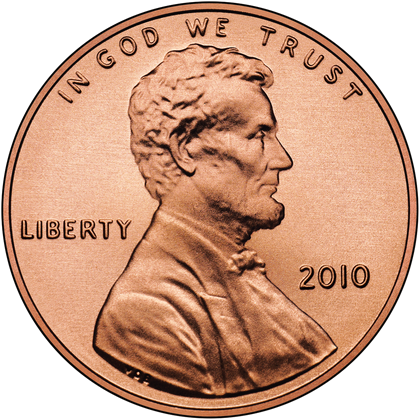
\includegraphics[width=0.84cm]{Figures/penny.png}};}
            \node[morange=5.3pt] at (-0.42,-0.75) {};
            \node[mgreen=5.3pt] at (-0.23,-0.75) {};
            \node[mgreen=5.3pt] at (-0.04,-0.75) {};
            \node[morange=5.3pt] at (0.15,-0.75) {};
            \node[mgreen=5.3pt] at (0.34,-0.75) {};
            \node[mgreen=5.3pt] at (1.78,-0.75) {};
            \node[morange=5.3pt] at (1.97,-0.75) {};
            \node[mgreen=5.3pt] at (2.16,-0.75) {};
            \node[morange=5.3pt] at (2.35,-0.75) {};
            \node[morange=5.3pt] at (2.54,-0.75) {};
            \node[mgreen=5.3pt] at (4.98,-0.75) {};
            \node[mgreen=5.3pt] at (5.17,-0.75) {};
            \node[mgreen=5.3pt] at (5.36,-0.75) {};
            \node[mgreen=5.3pt] at (5.55,-0.75) {};
            \node[mgreen=5.3pt] at (5.74,-0.75) {};
        \end{tikzpicture}
    \end{adjustbox}
\end{center}

\begin{eg}[Coin game]\label{eg:coin}
    Everyone in a size-\(150\) ML class flips a coin \(5\) times, and one of the
    students gets \(5\) heads for her coin `\(g\)'. Is `\(g\)' really magical?

    No. Even if all \(150\) coins are fair, the probability that \emph{one of
    them} results in \(5\) heads is
    \[
        1 - \left( \frac{31}{32} \right)^{150} > 99\% .
    \]
\end{eg}

A single fair coin gives five heads with probability \(\frac{1}{32}\), which is
small; \(150\) of them give it with probability \(99.1\%\), which is a near
certainty. Nothing about any individual coin changed. What changed is that we
were allowed to look at all \(150\) results and then name the coin --- and the
naming is the part Hoeffding says nothing about.

\begin{moral}
    BAD sample: \(\Ein\) and \(\Eout\) far away --- and it can get worse when
    `choice' is involved.
\end{moral}

\subsection{BAD Sample and BAD Data}

\begin{definition}[BAD sample, BAD data]\label{def:bad}
    A \vocab{BAD sample} is one on which \(\Ein\) and \(\Eout\) are far apart:
    \(\Eout = \frac{1}{2}\), say, but all heads came up, so \(\Ein = 0\).
    A data set \(\mathcal{D}\) is \vocab{BAD data for \(h\)} when
    \(\Eout(h)\) and \(\Ein(h)\) are far away --- for instance \(\Eout(h)\) big,
    so \(h\) is far from \(f\), while \(\Ein(h)\) is small, so \(h\) is correct
    on most of the examples.
\end{definition}

\begin{intuition}
    \autoref{thm:hoeffding-h} holds two things still and lets one vary. Held
    still are the distribution \(P\) on \(\mathcal{X}\) and the hypothesis
    \(h\); what varies is \(\mathcal{D}\), drawn i.i.d.\ from \(P\). In
    particular \(\Eout(h)\) does not move at all --- it is an expectation over
    \(P\), fixed by \(h\), \(f\) and \(P\) alone --- so every bit of the
    randomness sits in \(\Ein(h)\). The theorem is therefore a statement about
    the draw: however \(\mathcal{D}\) comes out, as long as \(N\) is large
    enough, \(\Ein(h)\) lands within \(\epsilon\) of that one fixed
    \(\Eout(h)\) --- for all but a \(2 \exp(-2 \epsilon^2 N)\) fraction of
    the possible \(\mathcal{D}\). Those rare exceptions are exactly the BAD
    data for \(h\).
\end{intuition}

That is the whole content of \autoref{thm:hoeffding-h}, restated as a property
of the data set rather than of a probability: Hoeffding says the BAD rows of the
following table are rare.

\begin{center}
    \begin{adjustbox}{max width=\textwidth}
        \solidrules
        \begin{tabular}{@{}c|cccccc|c@{}}
            \toprule
            & \(\mathcal{D}_1\) & \(\mathcal{D}_2\) & \(\dots\)
            & \(\mathcal{D}_{1126}\) & \(\dots\) & \(\mathcal{D}_{5678}\)
            & Hoeffding\\
            \midrule
            \(h\) & \textcolor{red!75!black}{\textbf{BAD}} & & & & &
            \textcolor{red!75!black}{\textbf{BAD}} &
            \(\mathbb{P}_{\mathcal{D}}\left[ \text{BAD } \mathcal{D}
            \text{ for } h \right] \le \dots\)\\
            \bottomrule
        \end{tabular}
    \end{adjustbox}
\end{center}

Reading a probability as a sum over data sets makes the next step obvious:
\[
    \mathbb{P}_{\mathcal{D}}\left[ \text{BAD } \mathcal{D} \right]
    = \sum_{\text{all possible } \mathcal{D}} \mathbb{P}(\mathcal{D}) \cdot
    \llbracket \text{BAD } \mathcal{D} \rrbracket ,
\]
and Hoeffding says this sum is small.

\subsection{BAD Data for Many \texorpdfstring{\(h\)}{h}}

With \(M\) hypotheses there are \(M\) rows, each with its own sparse scattering
of BAD entries, and the algorithm's freedom is exactly the freedom to avoid
them. Say that \(\mathcal{D}\) is \emph{BAD for many \(h\)} when it is BAD for
at least one of them; equivalently, when \(\mathcal{A}\) has no `freedom of
choice' on \(\mathcal{D}\), because there exists some \(h\) whose \(\Eout(h)\)
and \(\Ein(h)\) are far away.

\begin{center}
    \begin{adjustbox}{max width=\textwidth}
        \solidrules
        \begin{tabular}{@{}c|cccccc|c@{}}
            \toprule
            & \(\mathcal{D}_1\) & \(\mathcal{D}_2\) & \(\dots\)
            & \(\mathcal{D}_{1126}\) & \(\dots\) & \(\mathcal{D}_{5678}\)
            & Hoeffding\\
            \midrule
            \(h_1\) & \textcolor{red!75!black}{\textbf{BAD}} & & & & &
            \textcolor{red!75!black}{\textbf{BAD}} &
            \(\mathbb{P}_{\mathcal{D}}\left[ \text{BAD } \mathcal{D}
            \text{ for } h_1 \right] \le \dots\)\\
            \(h_2\) & & \textcolor{red!75!black}{\textbf{BAD}} & & & & &
            \(\mathbb{P}_{\mathcal{D}}\left[ \text{BAD } \mathcal{D}
            \text{ for } h_2 \right] \le \dots\)\\
            \(h_3\) & \textcolor{red!75!black}{\textbf{BAD}}
            & \textcolor{red!75!black}{\textbf{BAD}} & & & &
            \textcolor{red!75!black}{\textbf{BAD}} &
            \(\mathbb{P}_{\mathcal{D}}\left[ \text{BAD } \mathcal{D}
            \text{ for } h_3 \right] \le \dots\)\\
            \(\dots\) & & & & & & &\\
            \(h_M\) & \textcolor{red!75!black}{\textbf{BAD}} & & & & &
            \textcolor{red!75!black}{\textbf{BAD}} &
            \(\mathbb{P}_{\mathcal{D}}\left[ \text{BAD } \mathcal{D}
            \text{ for } h_M \right] \le \dots\)\\
            \midrule
            all & \textcolor{orange!85!black}{\textbf{BAD}}
            & \textcolor{orange!85!black}{\textbf{BAD}} & & & &
            \textcolor{orange!85!black}{\textbf{BAD}} & \(?\)\\
            \bottomrule
        \end{tabular}
    \end{adjustbox}
\end{center}

\begin{question}
    For \(M\) hypotheses, what bounds
    \(\mathbb{P}_{\mathcal{D}}\left[ \text{BAD } \mathcal{D} \right]\)?
\end{question}

\subsection{Bound of BAD Data}

\begin{theorem}[Finite-bin Hoeffding]\label{thm:finite-hoeffding}
    Let \(\mathcal{H} = \left\{ h_1, \dots , h_M \right\}\) be finite and let
    \(g\) be whatever \(\mathcal{A}\) returns. For every \(\epsilon > 0\),
    \[
        \mathbb{P}\left[ \abs{\Ein(g) - \Eout(g)} > \epsilon \right]
        \le 2M \exp \left( -2 \epsilon^2 N \right) .
    \]
\end{theorem}

\begin{proof}
    A data set on which \(g\) fails is a data set on which \emph{some} \(h_m\)
    fails, whichever \(h_m\) the algorithm happened to return, so
    \begin{align*}
        \mathbb{P}_{\mathcal{D}}\left[ \text{BAD } \mathcal{D} \right]
        &= \mathbb{P}_{\mathcal{D}}\left[ \text{BAD } \mathcal{D} \text{ for } h_1
        \text{ or } \dots \text{ or BAD } \mathcal{D} \text{ for } h_M \right]\\
        &\le \mathbb{P}_{\mathcal{D}}\left[ \text{BAD } \mathcal{D} \text{ for } h_1 \right]
        + \dots
        + \mathbb{P}_{\mathcal{D}}\left[ \text{BAD } \mathcal{D} \text{ for } h_M \right]
        \tag{union bound}\\
        &\le 2 \exp \left( -2 \epsilon^2 N \right) + \dots
        + 2 \exp \left( -2 \epsilon^2 N \right)\\
        &= 2M \exp \left( -2 \epsilon^2 N \right) ,
    \end{align*}
    the third line by \autoref{thm:hoeffding-h} applied to each fixed \(h_m\)
    separately.
\end{proof}

\begin{itemize}
    \item The finite-bin version is valid for all \(M\), \(N\) and \(\epsilon\).
    \item It does not depend on any \(\Eout(h_m)\), so there is no need to
        `know' them: \(f\) and \(P\) can stay unknown.
    \item `\(\Ein(g) = \Eout(g)\)' is PAC, \emph{regardless of} \(\mathcal{A}\).
\end{itemize}

\begin{remark}
    The union bound is crude --- it adds \(M\) probabilities as if the bad
    events never overlapped, when in a typical \(\mathcal{H}\) similar
    hypotheses fail on exactly the same data sets. Paying \(M\) for that
    crudeness is harmless while \(M\) is a few thousand and fatal when \(M\) is
    infinite. The next chapters buy the slack back.
\end{remark}

The last bullet is what makes the bound useful, because it frees the algorithm
completely: whatever rule \(\mathcal{A}\) uses to choose, the chosen \(g\) is
covered. And once every hypothesis is covered, the sensible thing to do is the
obvious thing.

\begin{moral}
    The `most reasonable' \(\mathcal{A}\), like PLA or pocket: pick the \(h_m\)
    with the lowest \(\Ein(h_m)\) as \(g\).
\end{moral}

\subsection{The `Statistical' Learning Flow}

Putting the two halves together gives the statement this chapter was after. If
\(\abs{\mathcal{H}} = M\) is finite and \(N\) is large enough, then for whatever
\(g\) is picked by \(\mathcal{A}\) we have \(\Eout(g) \approx \Ein(g)\); and if
\(\mathcal{A}\) finds one \(g\) with \(\Ein(g) \approx 0\), the PAC guarantee
gives \(\Eout(g) \approx 0\). Learning is possible.

\begin{center}
    \begin{adjustbox}{max width=\textwidth}
        \begin{tikzpicture}
            \node[mlbox, minimum width=4.4cm] (f) at (0,2.5)
                {unknown target function\\
                 \(f\colon \mathcal{X} \to \mathcal{Y}\)\\[2pt]
                 {\scriptsize (ideal credit approval formula)}};
            \node[mlbox, minimum width=2.6cm, draw=Dandelion!80!black,
                fill=Dandelion!12] (P) at (5.4,2.5)
                {unknown\\\(P\) on \(\mathcal{X}\)};
            \node[mlbox, minimum width=5.2cm] (D) at (0,0)
                {training examples\\
                 \(\mathcal{D}\colon (\bm{x}_1, y_1), \dots , (\bm{x}_N, y_N)\)\\[2pt]
                 {\scriptsize (historical records in bank)}};
            \node[mlop, minimum width=2.4cm] (A) at (5.4,0)
                {learning\\algorithm\\\(\mathcal{A}\)};
            \node[mlbox, minimum width=4.4cm] (g) at (10.2,0)
                {final hypothesis\\\(g \approx f\)\\[2pt]
                 {\scriptsize (`learned' formula to be used)}};
            \node[mlbox, minimum width=3.4cm] (H) at (5.4,-2.4)
                {hypothesis set\\\(\mathcal{H}\)\\[2pt]
                 {\scriptsize (set of candidate formulas)}};
            \draw[mlarrow] (f) -- (D);
            \draw[mlarrow, draw=Dandelion!80!black, dashed] (P) -- (D)
                node[pos=0.58, font=\scriptsize, fill=white, inner sep=1.5pt]
                {\(\bm{x}_1, \bm{x}_2, \dots , \bm{x}_N\)};
            \draw[mlarrow, draw=Dandelion!80!black, dashed] (P.east) -- (g.north)
                node[pos=0.55, font=\scriptsize, fill=white, inner sep=1.5pt]
                {\(\bm{x}\)};
            \draw[mlarrow] (D) -- (A);
            \draw[mlarrow] (A) -- (g);
            \draw[mlarrow] (H) -- (A);
            \node[right, font=\small, align=left, text=Dandelion!80!black]
                at (7.4,-2.4) {\(M = \infty\)? (like perceptrons)\\
                 ---see you in the next lectures};
        \end{tikzpicture}
    \end{adjustbox}
\end{center}

The catch is in the hypothesis of the theorem. \(M = \abs{\mathcal{H}}\) must be
finite, and the one hypothesis set we own --- the perceptrons of
\autoref{sec:perceptron-set} --- is a continuum. \autoref{thm:finite-hoeffding}
with \(M = \infty\) says nothing at all.

\begin{exercise}[Fun Time]
    Consider \(4\) hypotheses,
    \[
        h_1(\bm{x}) = \sign(x_1), \quad h_2(\bm{x}) = \sign(x_2), \quad
        h_3(\bm{x}) = \sign(-x_1), \quad h_4(\bm{x}) = \sign(-x_2).
    \]
    For any \(N\) and \(\epsilon\), which of the following statements is
    \emph{not} true?
    \begin{enumerate}[(1)]
        \item the BAD data of \(h_1\) and the BAD data of \(h_2\) are exactly
            the same;
        \item the BAD data of \(h_1\) and the BAD data of \(h_3\) are exactly
            the same;
        \item \(\mathbb{P}_{\mathcal{D}}\left[ \text{BAD for some } h_k \right]
            \le 8 \exp \left( -2 \epsilon^2 N \right)\);
        \item \(\mathbb{P}_{\mathcal{D}}\left[ \text{BAD for some } h_k \right]
            \le 4 \exp \left( -2 \epsilon^2 N \right)\).
    \end{enumerate}
\end{exercise}

\begin{proof}[Reference Answer]
    (1). Settle (2) first, because it decides everything else. Wherever
    \(x_1 \neq 0\) we have \(h_3(\bm{x}) = -h_1(\bm{x})\), and with
    \(\mathcal{Y} = \{+1, -1\}\) that means \(h_3\) is wrong exactly where
    \(h_1\) is right:
    \[
        \Ein(h_3) = 1 - \Ein(h_1), \qquad \Eout(h_3) = 1 - \Eout(h_1) .
    \]
    Subtracting, \(\Ein(h_3) - \Eout(h_3) = -\left( \Ein(h_1) - \Eout(h_1)
    \right)\). The two gaps have the same absolute value, so \(\mathcal{D}\) is
    BAD for \(h_3\) exactly when it is BAD for \(h_1\): (2) is true, and the
    same argument pairs \(h_4\) with \(h_2\).

    The four rows of the BAD table are therefore only two distinct rows, and the
    union bound has two terms to add rather than four:
    \[
        \mathbb{P}_{\mathcal{D}}\left[ \text{BAD for some } h_k \right]
        = \mathbb{P}_{\mathcal{D}}\left[ \text{BAD for } h_1 \text{ or BAD
        for } h_2 \right]
        \le 2 \cdot 2 \exp \left( -2 \epsilon^2 N \right) .
    \]
    That is (4), and (3) is a weaker bound, so it holds as well. Only (1) is
    left, and it fails: \(h_1\) and \(h_2\) read different coordinates of
    \(\bm{x}\), and nothing ties the examples one gets wrong to the examples
    the other gets wrong.

    The moral is worth keeping for the next chapter. Counting hypotheses
    overcounts BAD data as soon as two hypotheses go wrong on the same data
    sets --- here \(M = 4\) while the honest count is \(2\) --- and similar
    ideas will conquer the \(M = \infty\) case.
\end{proof}

\hrulebar

\subsection*{Summary}

\begin{description}
    \item[Learning is impossible?] Absolutely no free lunch outside
        \(\mathcal{D}\).
    \item[Probability to the rescue] Probably approximately correct outside
        \(\mathcal{D}\).
    \item[Connection to learning] Verification possible if \(\Ein(h)\) is small
        for a fixed \(h\).
    \item[Connection to real learning] Learning possible if \(\abs{\mathcal{H}}\)
        is finite and \(\Ein(g)\) is small.
\end{description}

The chapter's title keeps its question mark only for the first section. Learning
is impossible if the target is arbitrary and the guarantee must be certain; it
is possible as soon as we sample i.i.d.\ from a fixed \(P\) and accept a
guarantee that is probabilistic, with \(\Ein\) the quantity we minimise and
\(\Eout\) the quantity we are actually judged on.

What survives as a debt is the factor \(M\). It is the only place where the size
of \(\mathcal{H}\) enters, and it is the reason a bigger hypothesis set is not
free: more candidates make \(\Ein\) easier to drive down and make the bound
worse. The next chapter puts that trade-off at the centre --- and starts by
replacing \(M\) with something that stays finite even when \(\mathcal{H}\) does
not.
